
\section{Elektronische Transporteigenschaften} \label{sec:6}
In Kapitel 5: Stationäre SGL im TD GG $\rightarrow$ elektronische Zustände im Gitter. \\
Hier: Bewegung von Elektronen im Festkörper, z.B
\begin{itemize}
    \item elektrische Leitfähigkeit
    \item Wärmeleitfähigkeit
\end{itemize}
$\rightarrow$ zeitabhängige Probleme, System nicht im TD GG durch Anlgegen von äußeren Feldern (elektrisch o. magnetisch).

\subsection{Semiklassische Bewegungsgleichung von Ladungen in Bändern} \label{sec:6_1}
bisher: Elektronen als ausgedehnte Wellen (Bloch-Wellen) \\
hier: lokalisierte Elektronen für Transport:
\begin{itemize}
    \item Unschärferelation ($\Delta p \cdot \Delta x \ge \hbar$ oder $\Delta k \cdot \Delta x \ge 1$), d.h. räumliche Lokalisierung bedingt Unbestimmtheit des Wellenvektors.
    \item \textbf{freie Elektronen}: lineare Superposition von ebenen Wellen mit $k - \Delta k / 2 < k < k + \Delta k / 2$ führt auf \textbf{Wellenpakete}
          \begin{align}
              \Psi(\textbf{r},t) \propto \int_{k-\Delta k/2}^{k+\Delta k/2} a(\textbf{k}) e^{i(\textbf{k}\textbf{r} - \omega(\textbf{k})t)} \mathrm{d}\textbf{k}
          \end{align}

          \begin{figure}[H]
              \centering
              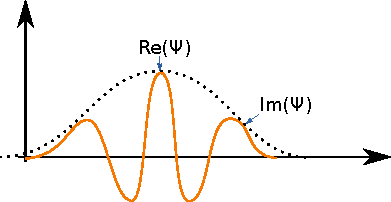
\includegraphics[width=0.8\textwidth]{figures/6_1Welle.pdf}
              \caption{}
              \label{fig:6_1Welle}
          \end{figure}

          Schwerpunkt des Pakets bewegt sich mit Gruppengeschwindigkeit $v_G = \left|\frac{\partial\omega(\textbf{k})}{\partial k}\right|$.
    \item \textbf{Im Kristall}: Superposition von Bloch-Wellen zu Wellenpaket: \\
          Wieder muss Unschärferelation gelten. Zusätzlich muss $\Delta k \ll \frac{\pi}{a}$ gelten, oder $\Delta x \gg a$, d.h. Wellenpaket dehnt sich über mehrere Elementarzellen aus. Bewegung des Elektrons (Wellenpakets) im äußeren Feld $\rightarrow$ Wellenlänge des Feldes $\lambda >> \Delta x$.

          \begin{figure}[H]
              \centering
              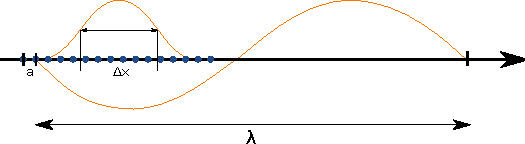
\includegraphics[width=0.8\textwidth]{figures/6_2BewEl.pdf}
              \caption{}
              \label{fig:6_1BewEl}
          \end{figure}

          Gruppengeschwindigkeit für das n-te Band: $\textbf{v}_n(\textbf{k}) = \nabla_\textbf{k} \omega(\textbf{k}) = \frac{1}{\hbar} \frac{\partial E_n(\textbf{k})}{\partial \textbf{k}} $ \\
          vorgehen: zeitabhängige SGL für nicht zu starke äußere Felder (vgl mit atomaren Feldern), die nicht zu stark räumlich und zeitlich variieren. $\rightarrow$ Theoretische Festkörperphysik \\
          hier: Semiklassische Bewegungsgleichung:
          \begin{align}
              \hbar \dot{\textbf{k}} = \textbf{F} = -e\left[\textbf{E}(\textbf{r},t) + \textbf{v}_n(\textbf{k}) \times \textbf{B}(\textbf{r},t)\right]
          \end{align}

          Analog zur Bewegungsgleichung freier Elektronen, aber mit $\textbf{v}_n(\textbf{k})$ und mit Quasiimpuls $\hbar \textbf{k}$ (nur bis auf $\textbf{G}$ festgelegt). Damit:
          \begin{align}
              \dot{\textbf{v}}_n = \frac{\partial}{\partial t} \left( \frac{1}{\hbar} \frac{\partial E_n(\textbf{k})}{\partial \textbf{k}} \right) =  \frac{1}{\hbar} \frac{\partial}{\partial \textbf{k}} \left( \frac{1}{\hbar} \frac{\partial E_n(\textbf{k})}{\partial \textbf{k}} \right) \cdot \hbar \cdot \frac{\partial \textbf{k}}{\partial t} = \frac{1}{\hbar^2} \frac{\partial^2 E_n(\textbf{k})}{\partial \textbf{k}^2} \cdot \textbf{F}
          \end{align}
          mit der inversen Masse $m\dot{v} = F$. \\
          \textbf{Definition:} \textbf{effektive Masse} $m^*$
          \begin{align*}
              \left(\frac{1}{m^*_n}\right)_{ij} (\textbf{k}) = \frac{1}{\hbar^2}\frac{\partial E_n(\textbf{k})}{\partial k_i\partial k_j} \\
              \text{mit $i,j$ = 1,2,3}
          \end{align*}

          \begin{itemize}
              \item Tensor
              \item Die inverse effektive Masse $\sim$ Krümmung der Energiedispersion des n-ten Bandes
              \item \textbf{k}-Abhängigkeit
              \item Wechselwirkung zwischen Elektron und Kristallpotential steckt in $m^*$: \\
                    BWGL: $\underline{\underline{m_n^*}} \cdot \dot{\textbf{v}}_n = \textbf{F}_i$ Impuls: $\underline{\underline{m_n^*}} \cdot \textbf{v}_n = \hbar \textbf{k}$ \\
                    d.h bei Kristallelektronen hängt Beschleunigung i.d.R von \textbf{k} ab, und Beschleunigung und Kraft müssen nicht parallel sein. \\
                    Für $\underline{\underline{m_n^*}}$ gilt: \\
              \item Tensor ist symmetrisch, d.h. $(\underline{\underline{m_n^*}})_{ij} = (\underline{\underline{m_n^*}})_{ji}$ bzw. für die Inversen.
              \item Tensor lässt sich auf Hauptachsen transformieren $\rightarrow$ 3 unabhängige Komponenten.\\
                    Spezialfälle:
                    \begin{itemize}
                        \item[1] effektive Masse längs Hauptachsen gleich groß $\rightarrow$ isotrope elektronische Eigenschafen
                        \item[2] quadratische Dispersion des Bandes $E_n(\textbf{k}) = E_0 + \frac{\hbar^2}{2m_n^*}(k_x^2 + k_y^2 + k_z^2)$ $\rightarrow$  konstantes $m_n^*$ ($\rightarrow$  in der Nähe der Bandextrema !)
                    \end{itemize}
              \item $m_n^* (\textbf{k})$ für isotropen Festkörper
              \item $m_n^*$ für Band mit quadratischer Dispersion
                    \begin{itemize}
                        \item[$\rightarrow$] in der Nähe der Bandextrema lassen sich Energieniveaus i.d.R. gut durch Paraboloide beschreiben
                        \item[$\rightarrow$] $m_n^*$ kann positiv oder negativ sein.
                              % \begin{figure}[H]
                              %     \centering
                              %     \includegraphics[width=0.8\textwidth]{figures/6_m_eff.png}
                              %     \caption{($\rightsquigarrow$ Krümmung des Bandes)}
                              %     \label{fig:6_m_eff.png}
                              % \end{figure}
                    \end{itemize}
          \end{itemize}
\end{itemize}



\subsection{Elektronen und Löcher} \label{sec:6_2}
Was ist Beitrag der Elektronen aus \textbf{einem} Band zur Stromdichte:
\begin{itemize}
    \item[Ann.:] Keine Interbandübergänge, d.h. angelegte Felder sind nicht stark genug, um das Band zu ändern ($n$ = const)
\end{itemize}
Stromdichte (Strom pro Quadratschnittsfläche)
\begin{align*}
    \mathrm{d}\textbf{j}_{(n)} = \frac{D(k)}{V} (-e \cdot v(\textbf{k})) \cdot \mathrm{d}^3k
\end{align*}
mit $e$ = \SI{1.6}{\cdot 10^{-19} C} und $D(k) = \frac{2V}{(2 \pi)^3}$ (vgl. Kap. \ref{kap:5_1}).
\begin{align*}
    \textbf{j}_{(n)} = -\frac{e}{V} \int D(k) \cdot f(E(\textbf{k}),T) \cdot \textbf{v}(\textbf{k}) \mathrm{d}^3k
\end{align*}
Ann.: $T$ = \SI{0}{K}, $f(E(\textbf{k}),T) = \Theta(E_F^0 - E(\textbf{k}))$ mit der Fermi-Energie $E_F^0$.
\begin{align*}
    \Rightarrow \quad \textbf{j}_{(n)} = - \frac{e V}{4V\pi^3} \int_0^{\textbf{k}E_F^0} \textbf{v}(\textbf{k}) \mathrm{d}^3k = - \frac{e}{4 \pi^3} \int_0^{\textbf{k}E_F^0} \frac{1}{\hbar} \underset{\begin{matrix}
        \uparrow \\
        \nabla_k E(\textbf{k})
    \end{matrix}}{\frac{\partial E (\textbf{k})}{\partial\textbf{k}}} \mathrm{d}^3k
\end{align*}

\begin{itemize}
    \item[(a)] \textbf{Vollständig besetztes Band:} \\
        $\rightarrow$ Integration über gesamte 1.BZ: \\
        Aus Symmetriegründen ist $\textbf{j} = 0$, d.h \textbf{vollständig besetzte Bänder tragen nicht zum Ladungstransport bei}. \\
        Begründung:
        \begin{itemize}
            \item[(i)] Kristall mit Inversionssymmetrie $E(\textbf{k}) = E(- \textbf{k})$ \\
                \begin{align}
                    \textbf{v}(\textbf{k}) = \frac{1}{\hbar} \frac{\partial E(\textbf{k})}{\partial \textbf{k}} = \frac{1}{\hbar} \frac{\partial E(-\textbf{k})}{\partial \textbf{k}} = - \textbf{v}(-\textbf{k})
                \end{align}
            \item[(ii)] Kristall ohne Inversionssymmetrie:\\
            Zeitumkehrinvarianz der SGL: $E(\textbf{k},\uparrow) = E(-\textbf{k},\downarrow) $, damit für $\uparrow$ und $\downarrow$ Elektronen $\textbf{v}(\textbf{k}) = - \textbf{v}(-\textbf{k})$
        \end{itemize}
    \item[(b)] \textbf{teilweise besetzes Band:}
        \begin{align}
            \textbf{j} &= \textcolor{red}{-} \frac{e}{4\pi^3} \underset{\begin{matrix}
                \text{\textcolor{red}{unbesetzte}}\\
                \text{\textcolor{red}{Zustände}}
            \end{matrix}}{\int} \frac{\partial E(\textbf{k}) }{\partial \textbf{k}} \mathrm{d}^3 k\\
             &= \frac{e}{4\pi^3} \left[    \underbrace{\int_\text{1. BZ} \frac{1}{\hbar} \frac{\partial E(\textbf{k}) }{\partial \textbf{k}} \mathrm{d}^3 k }_{=0}   -  \underset{\begin{matrix}
                \text{unbesetzte}\\
                \text{Zustände}
            \end{matrix}}{\int} \frac{1}{\hbar} \frac{\partial E(\textbf{k}) }{\partial \textbf{k}} \mathrm{d}^3 k \right] \\
             &= + \frac{e}{4 \pi^3} \underset{\begin{matrix}
                \text{unbesetzte}\\
                \text{Zustände}
            \end{matrix}}{\int} \frac{1}{\hbar} \frac{\partial E(\textbf{k})}{\partial \textbf{k}} \mathrm{d}^3 k = \textcolor{blue}{+} \frac{e}{4 \pi^3} \underset{\begin{matrix}
                \text{\textcolor{blue}{unbesetzte}}\\
                \text{\textcolor{blue}{Zustände}}
            \end{matrix}}{\int} \frac{1}{\hbar} \textbf{v}(\textbf{k}) \mathrm{d}^3 k\\
            &\neq 0 \quad \text{falls } \textbf{E} \text{ oder } \textbf{B} \text{ Feld anliegt, also System nicht in TD GG ist.}
        \end{align}
        $\rightsquigarrow$  mit 2 Betrachtungsmöglichkeiten
        \begin{itemize}
            \item[\textcolor{red}{\textcircled{1}}] Transport in teilweise gefüllten Bänderen wird von \textcolor{red}{Elektronen} auf \textcolor{red}{besetzten} Zuständen getragen. \textcolor{red}{$\rightsquigarrow$ für fast alle Bänder}
            
            \item[\textcolor{blue}{\textcircled{2}}] Transport in teilweise gefüllten Bändern wird von positiven Ladungsträgern \textcolor{blue}{(Defektelektronen, Löcher)} auf den mit Elektronen unbesetzten Zuständen getragen. $\rightsquigarrow$ fast volle Bänder
        \end{itemize}
        Nahe des Bandmaximums:
        \begin{figure}[H]
            \centering
            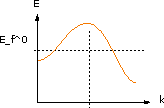
\includegraphics[width=0.8\textwidth]{figures/6_3Band.pdf}
            \caption{}
            \label{fig:6_3Band}
        \end{figure}
        \begin{align*}
            E(k) \approx E(k_0) + \frac{1}{2} &\underbrace{ \frac{\mathrm{d}^2E}{\mathrm{d}k^2}} (k-k_0)^2 \\
            &= \frac{\hbar^2}{m_e^*} = -\frac{\hbar^2}{|m_e^*|} (m_e^* < 0)
        \end{align*}
        damit:
        \begin{align*}
            \textbf{v}(\textbf{k}) &= \frac{1}{\hbar} \left(-\frac{\hbar^2}{|m_e^*|}(\textbf{k}-\textbf{k}_0)\right) \\
            \dot{\textbf{v}}(\textbf{k}) &= - \frac{\hbar \dot{\textbf{k}}}{|m_e^*|} \approx - \dot{\textbf{k}} \quad \text{d.h Beschleunigung entgegen ext. Kraft}
        \end{align*}
        \begin{align*}
            \text{d.h. } - |m_e^*| \cdot \dot{\textbf{v}}(\textbf{k}) &= - e (\textbf{E} + \textbf{v}(\textbf{k}) \times \textbf{B}) {\color{red} \quad \text{ BGL für Elektronen}} \\
         |m_e^*| \cdot \dot{\textbf{v}}(\textbf{k}) &= + e (\textbf{E} + \textbf{v}(\textbf{k}) \times \textbf{B}) \quad {\color{blue}\text{  BGL für Löcher}}
        \end{align*}
        \begin{figure}[H]
            \centering
            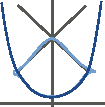
\includegraphics{figures/6_4Chaos.pdf}
            \caption{}
            \label{}
        \end{figure}
        \begin{table}[H]
            \centering
            \begin{tabular}{c|c|c}
                \textbf{Zusammenfassung:} & \textcolor{red}{Elektronen} & \textcolor{blue}{Löcher} \\ \hline \hline
                Ladung & -e & e \\
                eff. Masse & $m_e^* < 0$ & $m_h^* = - m_e^* > 0$ \\
                Wellenvektor & $\textbf{k}_e$ & $\textbf{k}_h = - \textbf{k}_e$ \\
                Energie & $E_e(\textbf{k}_e)$ & $E_h = - E_e(-\textbf{k}_e)$ \\
                Geschwindigkeit & $\textbf{v}_e(\textbf{k}_e)$ & $ \textbf{v}_h = \textbf{v}_e (- \textbf{k}_e)$ \\
                Spin & $\uparrow \downarrow$ & $ \downarrow \uparrow $
            \end{tabular}
        \end{table}
\end{itemize}



\subsection{Ladungstransport in Metallen} \label{sec:6_3}
\begin{itemize}
    \item[(a)] \textbf{Drude-Modell:}
    Ann.: Elektronen sind freie, klassische Teilchen
    \begin{itemize}
        \item[$\rightsquigarrow$] Bewegung mit therm. Geschwindigkeit $\textbf{v}_th$
        \item[$\rightsquigarrow$] Stöße mit Atomrümpfen in mittlerer Stoßzeit $\tau$
        \item[$\rightsquigarrow$] äußeres Feld \textbf{E} (oder \textbf{B}) 
        \item[$\rightsquigarrow$] Driftgeschwindigkeit $\textbf{v}_D = \textbf{v} - \textbf{v}_{th}$
    \end{itemize}
    BGL: $$ m^* \frac{\mathrm{d} \textbf{v}}{\mathrm{d}t} = - e \textbf{E} - m^* \frac{\textbf{v}_D}{\tau}$$ mit Driftgeschwindigkeit $\textbf{v}_D$ und der mittleren Stoßzeit $\tau$. Für Elektronen im Metall ist $m = m^*$\\
    Stationärer Zustand: $\frac{\mathrm{d} \textbf{v}}{\mathrm{d}t} = 0$
    $$\textbf{v}_D = - \frac{e \tau}{m} \cdot \textbf{E} = - \mu \textbf{E}$$ mit Beweglichkeit:
    \begin{center}
        \fbox{$\mu := \frac{e \tau}{m}$}\\
    \end{center}
    Stromdichte:
    \begin{align*}
        \textbf{j} = -e \cdot n \cdot \textbf{v}_D = \frac{n e^2 \tau}{m} \cdot \textbf{E} = n \cdot e \cdot \mu \cdot \textbf{E}
    \end{align*}
    mit elektrischer Leitfähigkeit \fbox{$\sigma = \frac{n e^2 \tau}{m} = n e \mu$}\\
    $\textbf{j} = \sigma \textbf{E}$ ist die mikroskopische Form des Ohmschen Gesetzes.\\
    $\sigma$ durch Materialparameter bestimmt. Für typische Metalle: $n \sim 10^{30}$ m$^{-3}$, $\tau \sim 10^{-14}$ s, damit $\sigma \sim 10^8 \frac{1}{\Omega \text{m}}$.\\
    z.B. bei 300 K:
    \begin{table}[H]
        \centering
        \begin{tabular}{r l}
            Ag: & $\sigma$ = \SI{6.1}{\cdot 10^7 (\Omega m)^{-1}}\\
            Cu: & $\sigma$ = \SI{5.8}{\cdot 10^7 (\Omega m)^{-1}}\\
            Au: & $\sigma$ = \SI{4.5}{\cdot 10^7 (\Omega m)^{-1}}
        \end{tabular}
    \end{table}

    Erfolge des Drude-Modells:
    \begin{itemize}
        \item DC Leitfähigkeit (Ohmsches Gesetz, siehe oben), AC Leitfähigkeit ($\sigma = \frac{n e^2 \tau}{m} \cdot \frac{1}{1-i\omega \tau}$)
        \item Hall-Effekt (B-Feld)
        \item Wiedemann-Frantz-Gesetz:\\
        Zusammenhang zwischen elektrischer und thermischer Leitfähigkeit $$\frac{K}{\sigma} = \frac{\pi^2}{3} \left(\frac{k_B}{e}\right)^2 \cdot T$$
        $\rightsquigarrow$ gute elektrische Leiter $\leftrightarrow$ gute Wärmeleiter
    \end{itemize}
    Problem (?): Im Drude Modell werden alle Leitungselektronen beschleunigt \& gestreut. Widerspruch zu Fermi-Dirac-Verteilungsfunktion

\item[(b)] \textbf{Sommerfeld Modell} ($\rightsquigarrow$ vgl. auch Kap. \ref{kap:5_1})
\begin{itemize}
    \item[Ann.:] Elektronen sind Quasiteilchen, quantenmechanische Teilchen $\rightarrow$ SGL, Pauli-Prinzip
    \item[$\rightarrow$] einfache Metalle (Alkali- und Edelmetalle)
    \item[$\rightarrow$] $\sim$ halb gefülltes Leitungsband
    \item[$\rightarrow$] Fermi-Fläche ist $\approx$ Fermi-Kugel
\end{itemize}
BGL unter E-Feld:
\begin{align*}
    \hbar \dot{\textbf{k}} = \dot{\textbf{F}} = - e \textbf{E} \quad \rightarrow \quad \text{\fbox{$\delta k = - \frac{e \textbf{E} \delta t}{\hbar}$}}
\end{align*}
Interpretation:
\begin{itemize}
    \item Bei \textbf{E} = 0 ist die Fermi-Kugel um \textbf{k} = 0 zentriert.
    \item Für \textbf{E} $\neq$ 0 verschiebt sich die gesamte Fermi-Kugel um $\delta$\textbf{k}.
\end{itemize}
% \begin{figure}[H]
%     \centering
%     \includegraphics[width=0.8\textwidth]{figures/5_fkugel_verschiebung.png}
%     \caption{}
%     \label{fig:5_fkugel_verschiebung.png}
% \end{figure}
\begin{itemize}
    \item Umverteilung von Elektronen von \textcolor{green}{///} nach \textcolor{blue}{///} durch Streuung
    \item Stationärer Zustand: Verschiebung der Fermilänge durch Relaxationszeit $\tau$ gegeben.
    \begin{center}
        \fbox{$\delta \textbf{k} = \frac{-e \textbf{E} \tau}{\hbar}$}
    \end{center}
    \item $\delta k / k_F \approx 10^{-7}$, d.h. $f-f_0 \neq 0$ nur in der Nähe von $k_F$
    \item Nur Elektronen in halbmondförmigen Bereichen tragen zur Leitfähigkeit bei.\\
    Kein Widerspruch zum Drude-Modell, denn:
    \begin{align*}
        \textbf{j}_{D = Drude} &= - e \cdot n \cdot \textbf{v}_D = + \frac{e \tau \textbf{E}}{m} \cdot \frac{\hbar \textbf{k}_F}{\hbar \textbf{k}_F}\\
        &= -e \cdot \tilde{n}\cdot \textbf{v}_F \qquad \text{mit} \quad \tilde{n} = n \cdot \frac{\delta \textbf{k}}{\textbf{k}_F}\\
        &= \textbf{j}_{S = Sommerfeld}
    \end{align*}
    $\tilde{n}$ gilt als an der Verschiebung beteiligte Ladungsträgerdichte.
\end{itemize}

Erfolge des Sommerfeld-Modells: Leitfähigkeit, Wiedemann-Frantz-Gesetz

\end{itemize}
